\documentclass[conference]{IEEEtran}
\IEEEoverridecommandlockouts
\usepackage[T1]{fontenc}
\usepackage{cite}
\usepackage{amsmath,amssymb,amsfonts}
\usepackage{algorithmic}
\usepackage{graphicx}
\usepackage{textcomp}
\usepackage{xcolor}
\usepackage{booktabs}
\usepackage{url}
% Hanging bullet for Table I cells: a plain paragraph per item aligns with the
% row baseline, which an itemize inside a p{} cell does not. The \par goes
% *before* the item: ending the cell with \par would push the array's final
% strut onto an empty extra line under every row.
\newcommand{\bl}[1]{\par{\hangindent=6pt\hangafter=1\noindent\textbullet\ #1}}

\let\IEEEoriginalcaption\caption
\renewcommand{\caption}[1]{\IEEEoriginalcaption{\footnotesize #1}}

% Single-column \figure floats default to plain LaTeX's stingy limits
% (topnumber=2, totalnumber=3), which pile up and defer to the end of
% the document once more than a couple of them are in flight at once.
% Loosen them so each figure can place near its own reference.
\renewcommand{\topfraction}{0.9}
\renewcommand{\textfraction}{0.07}
\renewcommand{\floatpagefraction}{0.7}
\setcounter{topnumber}{4}
\setcounter{bottomnumber}{3}
\setcounter{totalnumber}{6}

\renewcommand{\arraystretch}{0.92}

\setlength{\textfloatsep}{7pt plus 2pt minus 3pt}
\setlength{\intextsep}{7pt plus 2pt minus 3pt}
\setlength{\floatsep}{6pt plus 2pt minus 2pt}
\setlength{\abovecaptionskip}{4pt plus 1pt minus 1pt}
\setlength{\belowcaptionskip}{0pt}
\setlength{\dbltextfloatsep}{9pt plus 2pt minus 3pt}
\setlength{\dblfloatsep}{7pt plus 2pt minus 2pt}

\newcommand{\yes}{$\checkmark$}
\newcommand{\no}{$\times$}

\def\BibTeX{{\rm B\kern-.05em{\sc i\kern-.025em b}\kern-.08em
    T\kern-.1667em\lower.7ex\hbox{E}\kern-.125emX}}

\begin{document}

\title{Web2Music: Deployment-Level Measurement of Page-Conditioned Generative Audio in a Browser Extension}

\author{\IEEEauthorblockN{Ayush Kumar}
\IEEEauthorblockA{\textit{School of Computer Science} \\
\textit{and Engineering} \\
\textit{Vellore Institute of Technology}\\
Vellore, India \\
theofficialayush.kumar@gmail.com}
\and
\IEEEauthorblockN{Sneha Jakhotiya}
\IEEEauthorblockA{\textit{School of Computer Science} \\
\textit{and Engineering} \\
\textit{Vellore Institute of Technology}\\
Vellore, India \\
sneha.rajesh2025@vitstudent.ac.in}
\and
\IEEEauthorblockN{Vedant Vidhani}
\IEEEauthorblockA{\textit{School of Computer Science} \\
\textit{and Engineering} \\
\textit{Vellore Institute of Technology}\\
Vellore, India \\
vedant.vidhani2025@vitstudent.ac.in}
\and
\IEEEauthorblockN{Tvisha Thakur}
\IEEEauthorblockA{\textit{School of Computer Science} \\
\textit{and Engineering} \\
\textit{Vellore Institute of Technology}\\
Vellore, India \\
tvisha.thakur2025@vitstudent.ac.in}
\and
\IEEEauthorblockN{Pari Khandal}
\IEEEauthorblockA{\textit{School of Computer Science} \\
\textit{and Engineering} \\
\textit{Vellore Institute of Technology}\\
Vellore, India \\
pari.khandal2025@vitstudent.ac.in}
\and
\IEEEauthorblockN{Sixth Author}
\IEEEauthorblockA{\textit{School of Computer Science} \\
\textit{and Engineering} \\
\textit{Vellore Institute of Technology}\\
Vellore, India \\
email@vitstudent.ac.in}
}

\maketitle

\begin{abstract}
Generative audio models can produce plausible music from text, but
placing one inside an always-on browser extension raises problems audio
quality alone does not solve: deriving a prompt from a page, keeping
browsing history private, and hiding a slow generator from the critical
path. We present Web2Music and measure where these assumptions fail. A
four-signal page descriptor adds well under a tenth of a second per
page. A three-stage cascade (keyword, zero-shot NLI, LLM) barely moves accuracy across its confidence thresholds and, with a hosted middle
stage, never meaningfully reduces off-device disclosure. Fallback-then-swap
decouples audible start from generation, though some cold requests still
run long enough to time out. Across a corpus of real sites, requests and
generated clips we report five further negative results: a crossfade
that worsens a large share of seams; substantial loss of the requested
clip duration; a sensitive-content detector that misses most of an
adversarial slice; weak mood agreement among annotators; and an
engineered prompt that loses to a bare mood word on nearly every loop
metric.
\end{abstract}

\begin{IEEEkeywords}
generative audio, context-aware computing, browser extensions, zero-shot
classification, model cascades, on-device inference, ambient interfaces
\end{IEEEkeywords}

% ===========================================================================
\section{Introduction}
% ===========================================================================

Background music is chosen once, for a session, and then ignored: a lo-fi
playlist runs for four hours across a tax form, a horror wiki and a birthday
message without acknowledging that anything changed. It is context-free
because making it context-aware has historically required a human curator or
a library covering every context in advance. Text-conditioned generative
audio models remove that constraint in principle (\S\ref{sec:related}): if
the description can be derived from what the user is doing, the curator is
no longer needed.

\begin{table*}[!t]
\caption{Closest related systems.}
\label{tab:litreview}
\begin{center}
\scriptsize
\setlength{\tabcolsep}{4pt}
\begin{tabular}{p{0.95in}p{1.95in}p{1.6in}p{1.7in}}
\toprule
\textbf{Authors} & \textbf{Approach} & \textbf{Pros} & \textbf{Cons} \\
\midrule
Copet et al. \cite{musicgen} & MusicGen: single-stage transformer LM over EnCodec tokens &
\bl{Open; small variant deployable} &
\bl{One-shot clip, no loop closure}\bl{No context derivation} \\[1.5pt]
Agostinelli et al. \cite{musiclm} & MusicLM: hierarchical semantic/acoustic tokens &
\bl{Higher fidelity, long-form coherence} &
\bl{Heavy; not openly deployable}\bl{Non-looping} \\[1.5pt]
Liu et al. \cite{audioldm} & AudioLDM: latent diffusion on CLAP embeddings &
\bl{Faster than autoregressive tokens} &
\bl{Cost scales with sampling steps}\bl{No loop, no affect target} \\[1.5pt]
Agres et al. \cite{affectmachine} & AffectMachine-Pop: rule-based generation from a valence--arousal target &
\bl{Truly real time, no GPU}\bl{Interpretable} &
\bl{Affect target supplied externally, not derived from context} \\[1.5pt]
Liu et al. \cite{metabgm} & MetaBGM: two-stage LLM, game state $\to$ music description &
\bl{Fully automated}\bl{Multi-scene transitions} &
\bl{Full state to a cloud LLM every call}\bl{No listener study} \\[1.5pt]
Suzawa et al. \cite{discussionjockey} & Discussion Jockey 2: Whisper + GPT-4 descriptions $\to$ MusicGen &
\bl{Live context}\bl{User study raised relaxation} &
\bl{Full transcript to GPT-4 unfiltered}\bl{Small study} \\[1.5pt]
Wei et al. \cite{contextaitunes} & Context-AI Tunes: vision-LLM on a photographed scene + self-report &
\bl{Rigorous validation ($n=26$)} &
\bl{Scene image leaves the device}\bl{Active input} \\[1.5pt]
Chong et al. \cite{casper} & Casper: client-side rules $\to$ NER $\to$ LLM prompt sanitiser &
\bl{Fully client-side}\bl{Disclosure is the goal} &
\bl{Filters only, never generates}\bl{No corpus exposure rate} \\[1.5pt]
Chen et al. \cite{frugalgpt} & FrugalGPT: confidence-gated cascade before expensive LLMs &
\bl{Cascade pattern this paper adopts} &
\bl{Optimises cost/latency only}\bl{Never reports disclosure} \\[1.5pt]
\midrule
Web2Music (this paper) & Passive page context $\to$ 3-stage abstaining classifier $\to$ MusicGen behind fallback-then-swap &
\bl{Passive, not a request}\bl{Disclosure measured as a rate}\bl{Latency and failure modes measured} &
\bl{Perceptual benefit untested}\bl{Hosted cascade still discloses most pages} \\
\bottomrule
\end{tabular}
\end{center}
\end{table*}

Deriving it is where the engineering lives, via three constraints, none
about audio quality. \emph{The prompt has to come from somewhere:} a page
is a DOM of navigation chrome, ads and colour, not a prompt.
\emph{Classification is a privacy decision:} the most accurate way to
classify a page is an LLM call, but doing that on every page turns a music
player into a browsing-history exfiltration channel. \emph{The model is
too slow for the critical path:} on a CPU laptop the three cold requests
that completed took a median of 139 s for a 10--20 s clip, and every 28 s
cold request exceeded a 300 s client timeout, against a page load of about
two seconds -- a gap CPU inference does not close; the interaction must be
designed so it is invisible.

This paper's contributions follow the same three constraints. First, a
four-signal page descriptor (text, sentence embedding, page
colour, browsing behaviour) with its extraction cost measured over 105 real
websites; an offline ablation under the keyword stage bounds colour's effect
on the mood label at $\leq 7.5$ percent of pages and is uninformative for
the other two auxiliary signals (\S\ref{sec:res-signal-ablation}).

Second, an abstaining three-stage classifier (free keyword heuristic $\to$
zero-shot NLI $\to$ remote LLM) and the finding that, with a hosted cheap
stage, such a cascade \emph{redistributes} disclosure between providers
rather than reducing it: the thresholds are a privacy mechanism only if
the middle stage is local, which we measure only on an 18-page subset.

Third, a latency-hiding playback design: instant fallback followed by an
abort-on-stale crossfaded swap, with its full latency distribution and
failure modes, including 12 of 144 client timeouts; and loop synthesis
from a non-loop model, bar-snapped chroma self-similarity, a 50 ms
crossfade, and a gapless Ogg/Opus container, evaluated over 141 clips.

% ===========================================================================
\section{Related Work}
\label{sec:related}
\label{sec:recent-systems}
% ===========================================================================

\emph{Generative audio.} MusicGen \cite{musicgen} is a single-stage
transformer language model over discrete EnCodec \cite{encodec} tokens,
text-conditioned and openly deployable, which is why its small variant is
the generator here; MusicLM \cite{musiclm} and AudioLDM \cite{audioldm}
trade fidelity against speed, and AudioGen \cite{audiogen} applies the
same conditioning to environmental sound. All four emit a fixed-length
one-shot excerpt whose end does not join its beginning. AffectMachine-Pop
\cite{affectmachine} is rule-based and truly real time, but takes its
valence--arousal target \cite{russell} from outside rather than from
context.

\emph{Context-aware music and disclosure.} Four recent systems derive
music from a user's situation: MetaBGM \cite{metabgm} from game state,
Discussion Jockey 2 \cite{discussionjockey} from live meeting speech,
Context-AI Tunes \cite{contextaitunes} from a photographed scene plus
self-reported stress, and, on the privacy side, Casper \cite{casper}
sanitises a typed prompt with a client-side cascade before it reaches a
web LLM. FrugalGPT \cite{frugalgpt} established the confidence-gated
cascade pattern this paper's classifier follows, framed as cost and
latency optimisation. Table \ref{tab:litreview} places these against
Web2Music on the properties this paper measures.

Web2Music combines three properties no recent system in Table
\ref{tab:litreview} combines. \emph{Passive context, not a request:}
unlike MetaBGM, Discussion Jockey 2 and Context-AI Tunes, which respond
to something a user is actively doing, Web2Music's context is whatever
page is open, sensed without prompting. \emph{Disclosure as a measured
rate:} every system in Table \ref{tab:litreview} sends its full context
to a cloud model and reports no on-device fraction; Web2Music still
discloses most pages as measured (\S\ref{sec:res-classification}), but
the number is reported rather than assumed away. \emph{Deployment
failure modes as findings:} none of the four context-to-music papers
reviewed reports a latency distribution, cache behaviour, loop-continuity
measurement or adversarial audit. The contribution is accordingly the
deployment measurement -- not a better generator, classifier or cascade,
all three adopted from existing work -- and the finding that several
resulting guarantees do not hold as configured.

% ===========================================================================
\section{Research Gaps and Problem Statement}
\label{sec:gaps}
% ===========================================================================

\subsection{Gaps}

Prior work leaves four gaps, none about audio quality.
\emph{Deployment-level properties go unmeasured:} prompt cost,
generation-time behaviour and safeguard robustness fall outside the
audio-quality frame prior work uses. \emph{On-device classification is
treated as a cost problem, not a disclosure one:} no work we reviewed
reports an \emph{exposure rate} as a tunable curve. \emph{Context-aware
music systems assume a library:} whether generation beats retrieval on
cost is asserted, not measured. \emph{Generative audio models do not
produce loops:} how much a crossfade removes is not characterised in the
literature we found.

\subsection{Problem statement}

Given a rendered page $p$, produce ambient audio $a(t)$ appropriate to
$p$, subject to \emph{latency} (audible start bounded by the confidence
window plus under a second, independent of generation time),
\emph{disclosure} (text leaving the device is measurable and zero for
sensitive pages), \emph{continuity} (a clip repeats without an audible
seam), and \emph{restraint} (identifiable page classes get no output,
verifiably).

Five verdicts: fallback-then-swap keeps time-to-audio within budget
(\emph{supported}, \S\ref{sec:res-latency}); generation covers a request
space retrieval does not (\emph{argued only under a random-library model},
\S\ref{sec:res-retrieval}); loop synthesis reduces seam discontinuity
(\emph{gapless achieved, seam reduction marginal}, \S\ref{sec:res-loop});
restraint policies fire correctly (\emph{mechanism passes, detection
fails}, \S\ref{sec:res-audit}); the cascade reduces exposure at a
measurable cost (\emph{negative for the hosted backend},
\S\ref{sec:res-classification}).

% ===========================================================================
\section{System Architecture}
\label{sec:arch}
% ===========================================================================

Web2Music is a Manifest V3 Chrome extension plus one HTTP
audio-generation service. Fig.~\ref{fig:system} follows one page from DOM
to speaker in nine numbered steps and marks the two persistent stores
where they are touched: an IndexedDB vector store on the device and a
Postgres cache index behind the generation service. The division of
labour follows browser security boundaries: the descriptor extractor runs in the content script to reach
the DOM, the classifier runs in the service worker since the content
script's origin is untrusted, and playback and ONNX inference run in an
offscreen document since Manifest V3 forbids audio in a service worker
and a page's CSP blocks WebAssembly there. Three components are network
services: the hosted zero-shot backend, the remote LLM, and the
generation service.

\begin{figure}[!t]
\centerline{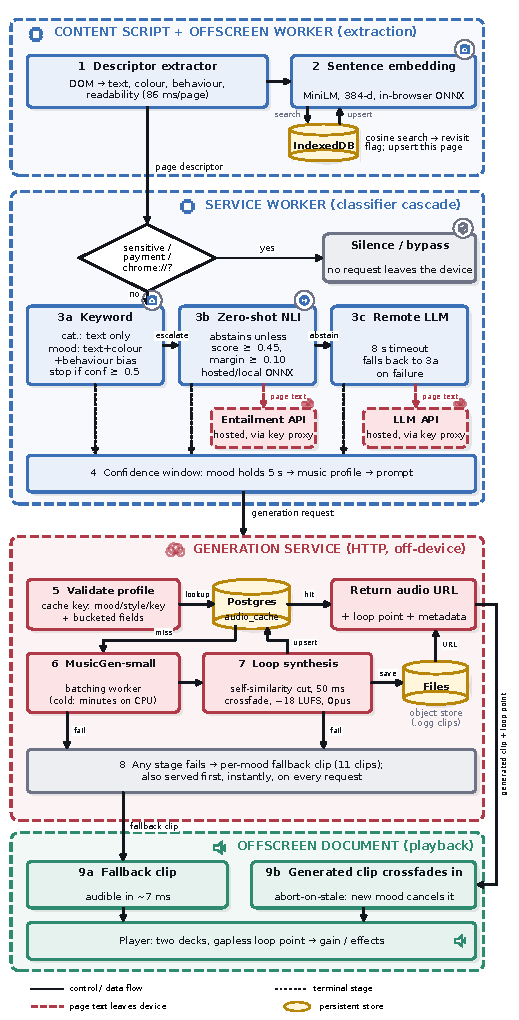
\includegraphics[width=\columnwidth]{figures/system.pdf}}
\caption{System architecture diagram.}
\label{fig:system}
\end{figure}

\subsection{Page descriptor extraction}

A single function assembles the descriptor from four contextual signals
-- text, a 384-dimensional MiniLM sentence embedding (in-browser ONNX),
colour (an area-weighted HSL histogram over up to 800 elements
\cite{dominantcolour}), and behaviour (scroll/cursor velocity) -- plus
readability \cite{flesch} as an auxiliary feature. The embedding is
searched by cosine similarity against an IndexedDB vector store of prior
pages (step 2 in Fig.~\ref{fig:system}) to flag a revisit, then upserted,
capped at 2,000 entries; this search is the vector-store row of Table
\ref{tab:extraction}. The embedding feeds the vector store only, not the
keyword stage's mood computation (\S\ref{sec:res-signal-ablation}
depends on this). Extraction stays off
the critical path: debounced, idle-scheduled, and re-run on navigation
and DOM mutation.

\subsection{Classification and the cascade}
\label{sec:res-classification}

Table \ref{tab:tiers} reports the cascade ablation and threshold sweep
across the ablation corpus.

\begin{table}[t]
\caption{Cascade configurations. Accuracy/F1 over 254 labelled pages;
exposure/disclosure over 260 records. Last two columns re-score against
the annotator majority on 208 pages; A2 has no re-scored figure.}
\label{tab:tiers}
\begin{center}
\scriptsize
\setlength{\tabcolsep}{2.5pt}
\begin{tabular}{lrrrrrrr}
\toprule
& & & \textbf{LLM} & \textbf{ZS} & \textbf{Total} & \multicolumn{2}{c}{\textbf{Re-scored}} \\
\textbf{Configuration} & \textbf{Acc.} & \textbf{F1} & \textbf{exp.} & \textbf{proxy} & \textbf{off-dev.} & \textbf{Acc.} & \textbf{F1} \\
\midrule
A1 keyword only & .189 & .315 & 0 & 0 & 0 & .197 & .297 \\
A2 zero-shot only & .520 & .562 & 0 & .938 & .938 & --- & --- \\
A3 LLM only & .685 & .678 & 1.00 & 0 & 1.00 & .764 & .731 \\
A4 keyword$\to$LLM & .669 & .677 & .762 & 0 & .762 & .760 & .705 \\
A5 keyword$\to$ZS$\to$LLM & .622 & .656 & .250 & .512 & .762 & .683 & .683 \\
\bottomrule
\end{tabular}
\end{center}
\end{table}

The full cascade (A5) falls behind keyword-to-LLM (A4) by 4.7 accuracy
points against the corpus labels, and by 7.7 points when re-scored
against the annotator majority (below). On the face of it, A5 sends far
fewer pages to the LLM than A4 does, .250 against .762. The catch is
that A5's zero-shot stage is itself a hosted, off-device call: every
page that would have reached the LLM in A4 is sent to the zero-shot
proxy in A5 first. Both configurations therefore have the same total
off-device rate of .762, and the cascade only decides which provider
receives a page's text. A5 is dominated, with lower accuracy at
identical disclosure, and would be worth running only with a local
middle stage, which we did not test at full scale.

\begin{figure}[tb]
\centerline{
\includegraphics[width=\columnwidth]{figures/f5.pdf}}
\caption{Macro-F1 against total off-device rate for A1--A5 and a
twelve-cell threshold sweep. Filled points (total off-device) stack at
.762 regardless of threshold; hollow points (LLM-only exposure) spread
.13--.60.}
\label{fig:f5}
\end{figure}

The threshold sweep shows this is not specific to the shipped operating
point. Macro-F1 ranges only from .653 to .668 and LLM exposure from .131
to .596, yet total off-device rate stays within .001 of .762 throughout.
\emph{Re-scoring against the annotator majority.} Category agreement
among annotators is $\alpha=0.635$, below the 0.667 reliability
threshold, so the majority vote is the better of two imperfect labels
rather than validated ground truth. On the 208 pages where the vote
resolves, the accuracy gap between A4 and A5 widens to 7.7 points
(95\% CI [2.9, 12.5], $p<0.01$), and the disclosure picture does not
change.

\subsection{Loop quality}
\label{sec:res-loop}

The loop-quality table (Table \ref{tab:seam}) reports objective loop
metrics over 141 generated clips.

\begin{table}[t]
\caption{Loop quality, 141 clips, 50 ms crossfade.}
\label{tab:seam}
\begin{center}
\scriptsize
\begin{tabular}{lrr}
\toprule
\textbf{Measure} & \textbf{p50} & \textbf{p95} \\
\midrule
Seam energy diff., pre-crossfade (dB) & 3.73 & 14.15 \\
Seam energy diff., post-crossfade (dB) & 2.64 & 10.77 \\
Paired improvement (dB)$^{\dagger}$ & 0.93 & --- \\
Clips worsened by the crossfade & \multicolumn{2}{r}{41.1\%} \\
Spectral centroid diff., pre / post (Hz) & 441 & 557 \\
Loudness (LUFS; target $-18.0$) & $-18.09$ & --- \\
Duration retention & 0.503 & 0.923 \\
\bottomrule
\end{tabular}
\end{center}
{\scriptsize $^{\dagger}$Median of per-clip differences, not the
difference of the two medians above.}
\end{table}

Loudness compliance is exact; the seam-continuity claim is not
supported. The crossfade helps less than expected. Median paired
improvement is 0.93 dB, and the crossfade worsens the energy seam on
41.1 percent of clips; on spectral centroid it is worse than nothing at
the median (441 Hz before, 557 after). On a secondary sample of ten
fallback clips, widening the crossfade to 500 ms only reduced median
discontinuity from 3.46 to 2.90 dB, while choosing the loop point that
minimises measured seam rather than trusting chroma similarity cut it
to 0.33 dB -- suggestive that the cut point, not the crossfade, is the
weaker link, though at $n=10$, unvalidated perceptually, and not on the
same clips as Table \ref{tab:seam}. Table \ref{tab:crossfade} gives the
full sweep.

\begin{table}[t]
\caption{Crossfade-window sweep, 11 persisted fallback clips ($n=10$
usable; one too short for the 500 ms window), production loop point
held fixed. Not the 141 generated clips of Table \ref{tab:seam}, which
is why the 50 ms row here does not match that table's post-crossfade
figure. Seam values are absolute differences at the loop seam,
post-crossfade.}
\label{tab:crossfade}
\begin{center}
\scriptsize
\begin{tabular}{lrr}
\toprule
\textbf{Crossfade width} & \textbf{$|\Delta E|$ p50 (dB)} & \textbf{$|\Delta$cent.$|$ p50 (Hz)} \\
\midrule
50 ms & 3.46 & 577 \\
100 ms & 3.10 & 343 \\
250 ms & 2.94 & 125 \\
500 ms & 2.90 & 195 \\
50 ms, seam-min.\ loop & 0.33 & --- \\
\bottomrule
\end{tabular}
\end{center}
\end{table}

Half the requested audio is discarded. Delivered clips retain a median
of 50.3 percent of requested duration: 28 s yields about 14 s. The
smallest retention (10.6 percent) is not a bug -- the source was
shorter than the 3.0 s minimum loop, so the whole clip looped.
Audibility is unanswered: a listening harness (22 seeded pairs) has
been validated only against simulated listeners. The self-similarity
cut, then, discards half the requested audio for a seam quality it
does not reliably predict; a generator conditioned to produce
loop-closed material directly would remove the problem rather than
patch it.

\subsection{Does the engineered prompt earn its cost?}
\label{sec:res-prompt}

The shipped prompt is an artificially constructed 300-character
description. Table \ref{tab:prompt} holds mood, duration and seed
fixed and varies only the prompt across three conditions: P1, the
bare mood word; P2, the service's own template; P3, the engineered
prompt production sends. Three generations of each of five moods, no
errors, no fallbacks.

\begin{table}[t]
\caption{Prompt ablation, $n=15$/condition, 15 s clips. Objective metrics
only.}
\label{tab:prompt}
\begin{center}
\scriptsize
\setlength{\tabcolsep}{2.5pt}
\begin{tabular}{lrrrr}
\toprule
\textbf{Prompt} & \textbf{chars} & \textbf{$|\Delta E|$ dB} & \textbf{$|\Delta$cent.$|$ Hz} & \textbf{Reten.} \\
\midrule
P1 bare mood & 5 & 3.75 & 565 & 0.527 \\
P2 template & 175 & 2.63 & 509 & 0.444 \\
P3 engineered & 312 & 4.35 & 316 & 0.393 \\
\bottomrule
\end{tabular}
\end{center}
\end{table}

On these numbers the engineered prompt doesn't earn its extra length:
it comes out worst on the energy seam, lowest on retention, and ahead
of the other two prompts only on the spectral-centroid seam. Prompt
length did not change generation time. This is objective-only at
$n=15$/cell -- a prompt can lose on every number here and still be
preferred by a listener -- and is reported as a negative result
pending the listening study, not as grounds to change the prompt.

\subsection{Restraint policies}
\label{sec:res-audit}

The fourteen executable behavioural policies -- sensitive-page
silence, mute/duck around existing audio, payment and
browser-internal bypass, a hashed-URL telemetry guarantee, and seven
direct-assertion unit cases -- all pass their mechanism-level tests;
the predicate behind the first of them does not. Table
\ref{tab:restraint} lists all fourteen policies and their covering
tests -- this audits the mechanisms, not the predicate, which Table
\ref{tab:sensitive} audits separately on a 47-page adversarial slice
below.

\begin{table}[t]
\caption{Restraint audit: the fourteen executable behavioural policies
and their covering tests. All fourteen pass. This audits the
mechanisms; the sensitive-content predicate they depend on is audited
in Table \ref{tab:sensitive}.}
\label{tab:restraint}
\begin{center}
\scriptsize
\begin{tabular}{p{3.2cm}p{4.0cm}}
\toprule
\textbf{Policy} & \textbf{Trigger / covering test} \\
\midrule
Crisis/sensitive $\to$ silence & one severe term, or two distinct ambiguous terms \\
Sensitive text skips LLM tiers & short-circuits both escalation paths \\
No competing with active audio & active tab audible gives mute; background gives duck \\
Payment/checkout bypassed & pattern match on URL and title \\
Browser-internal bypassed & pattern match on URL scheme \\
No plaintext history stored & every event stores a SHA-256 URL hash \\
Model-pin change detectable & golden fixtures re-checked against the pinned model \\
Seven unit cases$^{\dagger}$ & direct assertion, one per case \\
\bottomrule
\end{tabular}
\end{center}
{\scriptsize $^{\dagger}$Payment page detected; a non-payment page is
not flagged; \texttt{chrome://} bypassed; active audible tab gives
mute; background audible tab gives duck; silent browsing gives no
attenuation; silent media site gives duck, never mute.}
\end{table}

\begin{table}[t]
\caption{Sensitive-content audit, 47-page slice.}
\label{tab:sensitive}
\begin{center}
\scriptsize
\begin{tabular}{lr}
\toprule
\textbf{Metric} & \textbf{Result} \\
\midrule
Slice: sensitive / non-sensitive & 29 / 18 \\
False-negative rate & 19/29 = .655 \\
False-positive rate & 3/18 = .167 \\
Silence delivered on sensitive pages & 34.5\% \\
\bottomrule
\end{tabular}
\end{center}
\end{table}

The failures are systematic:
\begin{itemize}
\item Seven of nineteen misses use vocabulary outside the term list
(addiction, miscarriage, terminal illness, overdose, and similar);
\item Four fail because they rely on euphemism;
\item Four are non-English, which the English-vocabulary term lists
cannot match -- the check runs before any language gate, so this is a
coverage gap, not an ordering one;
\item A further four mention only one of the two required ambiguous
terms.
\end{itemize}
All three false positives are near-miss academic content (a
grief-counselling degree programme, a psychology textbook, an
engineering article using ``trauma''), unchanged as the slice grew.
\emph{Consequence.} A missed sensitive page is not silenced -- it goes
through the cascade like any other, reaching a hosted stage at the
corpus-wide .762 rate. The disclosure constraint of \S\ref{sec:gaps}
-- zero for sensitive pages -- holds only for the 34.5 percent of
sensitive pages the detector actually flags. This is a negative
result invisible to any evaluation that tests only whether the
mechanism fires; the remedy is a classifier, not more keywords.

\subsection{Generation against retrieval}
\label{sec:res-retrieval}

The request space is $11\times7\times5\times5=1{,}925$ cells. Fig.
\ref{fig:f7} is an analytical model, not a measurement: no library was
built. Under a uniformly distributed random-library model a 500-track
library covers under a quarter of the space, and roughly 5,000 tracks
are needed for 90 percent coverage, dropping to 55 percent under
skewed commissioning. The claim this supports is narrow -- coverage
grows slowly with library size under this model -- not that
generation covers a space retrieval cannot. By construction, a
curated 1,925-track library would reach 100 percent coverage, matching
every cell exactly. But exact-cell matching asks for more precision
than the data supports: annotators themselves agree on mood at only
$\alpha=0.195$, so treating every cell as a distinct target overstates
what is actually needed.

\begin{figure}[tb]
\centerline{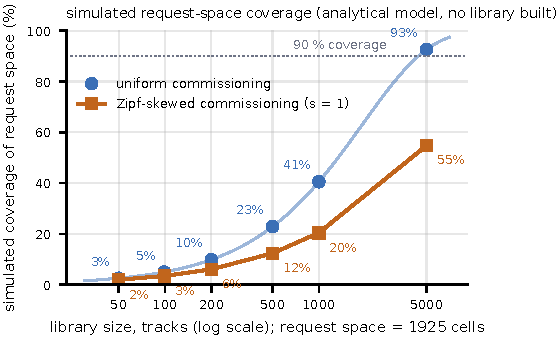
\includegraphics[width=\columnwidth]{figures/f7.pdf}}
\caption{Simulated coverage against library size, uniform and skewed
commissioning. Analytical, not empirical.}
\label{fig:f7}
\end{figure}

% ===========================================================================
\section{Conclusion}
% ===========================================================================

Web2Music surfaces where its own deployment assumptions fall short.
The four-signal descriptor runs at a median of 86 ms, and of the four
signals only colour is shown to move the mood label offline. The
three-stage abstaining classifier costs about 1.3 cents per thousand
pages, but it shifts disclosure between providers rather than reducing
it, and is outperformed by the simpler keyword-to-LLM design at the
same level of disclosure. Fallback-then-swap separates a 6.9 s
audible start from a generator with a median runtime of 139 s across
the three requests that completed, while 12 of 144 requests timed
out. Loop synthesis produces gapless output but not seamless output:
the crossfade worsens 41.1\% of seams, and only half of the requested
audio survives the search for a loop point. The sensitive-content
detector misses 65.5\% of an adversarial slice, so most sensitive
pages in it would still reach a hosted model. Three annotators agree
on mood at only $\alpha=0.195$. The engineered prompt also performs
worse than both the bare mood word and the service's own template on
most objective loop metrics. The core perceptual hypothesis -- that
page-conditioned music fits a page better than page-agnostic music --
remains untested.

% ===========================================================================
\section{Limitations and Future Work}
\label{sec:limitations}
% ===========================================================================

Testing this claim requires ethical approval. We plan a
within-subjects, counterbalanced comparison in which participants
judge how well matched and shuffled versions of the same audio fit,
rated on a Likert scale. Alongside this, we track two behavioural
measures: (i) dwell time, how long a listener stays on each clip, and
(ii) how often they skip or mute a clip. The instrument itself is
built; it is only ethical approval that remains outstanding. A null
result here would undercut this paper's premise.

The measurements carry real limits. Generation delay rests on only
three completed runs, and no 28 s cold generation finished inside the
client timeout. Client-side and embedding delay figures are both
stubbed, so they're floor values rather than true costs. The signal
ablation runs offline and only at the keyword level, which by design
tells us nothing about behaviour or the embedding. Mood accuracy
itself was never computed -- every accuracy figure reported is for
category, even though mood is what actually drives the music. The
three annotators were also the three authors, with no calibration
phase. The retrieval comparison assumes a random library and takes
the generator's prompt compliance on faith, without verifying it.
Loop-point selection was optimised against the same metric it is
evaluated on, using only $n=10$. The sensitive detector's 65.5\%
false-negative rate, which includes every non-English case, is a
real defect that needs fixing with a model-based predicate -- likely
the entailment step already in the extension -- before any
deployment, not something to just note in passing. The local
classification system that could reduce, rather than merely
redistribute, disclosure has so far only been tested on 18 pages,
against a corpus that escalates at .762 -- this is the highest-value
item still outstanding. The bigger opportunity in loop synthesis is
optimising the generator itself to produce loop-closed audio directly.
The same descriptor-to-profile pipeline could extend to other
continuous interfaces, like code or document editors.
\scriptsize
\begin{thebibliography}{00}

\bibitem{musicgen} J. Copet, F. Kreuk, I. Gat, T. Remez, D. Kant, G. Synnaeve, Y. Adi, and A. D\'efossez, ``Simple and controllable music generation,'' in \emph{Advances in Neural Information Processing Systems}, 2023.

\bibitem{encodec} A. D\'efossez, J. Copet, G. Synnaeve, and Y. Adi, ``High fidelity neural audio compression,'' \emph{Transactions on Machine Learning Research}, 2023.

\bibitem{musiclm} A. Agostinelli, T. I. Denk, Z. Borsos, J. Engel, M. Verzetti, A. Caillon, Q. Huang, A. Jansen, A. Roberts, M. Tagliasacchi, M. Sharifi, N. Zeghidour, and C. Frank, ``MusicLM: Generating music from text,'' arXiv:2301.11325, 2023.

\bibitem{audiogen} F. Kreuk, G. Synnaeve, A. Polyak, U. Singer, A. D\'efossez, J. Copet, D. Parikh, Y. Taigman, and Y. Adi, ``AudioGen: Textually guided audio generation,'' in \emph{Proc. Int. Conf. Learning Representations}, 2023.

\bibitem{audioldm} H. Liu, Z. Chen, Y. Yuan, X. Mei, X. Liu, D. Mandic, W. Wang, and M. D. Plumbley, ``AudioLDM: Text-to-audio generation with latent diffusion models,'' in \emph{Proc. Int. Conf. Machine Learning}, 2023.

\bibitem{affectmachine} K. R. Agres, A. Dash, P. Chua, and S. K. Ehrlich, ``AffectMachine-Pop: A controllable expert system for real-time pop music generation,'' arXiv:2506.08200, 2025.

\bibitem{russell} J. A. Russell, ``A circumplex model of affect,'' \emph{Journal of Personality and Social Psychology}, vol. 39, no. 6, pp. 1161--1178, 1980.

\bibitem{frugalgpt} L. Chen, M. Zaharia, and J. Zou, ``FrugalGPT: How to use large language models while reducing cost and improving performance,'' arXiv:2305.05176, 2023.

\bibitem{dominantcolour} Y. Chang and N. Mukai, ``Color feature based dominant color extraction,'' \emph{IEEE Access}, vol. 10, pp. 93055--93061, 2022.

\bibitem{flesch} R. Flesch, ``A new readability yardstick,'' \emph{Journal of Applied Psychology}, vol. 32, no. 3, pp. 221--233, 1948.

\bibitem{foote} J. Foote, ``Automatic audio segmentation using a measure of audio novelty,'' in \emph{Proc. IEEE Int. Conf. Multimedia and Expo}, 2000, pp. 452--455.

\bibitem{librosa} B. McFee, C. Raffel, D. Liang, D. P. W. Ellis, M. McVicar, E. Battenberg, and O. Nieto, ``librosa: Audio and music signal analysis in Python,'' in \emph{Proc. Python in Science Conf.}, 2015, pp. 18--25.

\bibitem{ebu128} European Broadcasting Union, ``Loudness normalisation and permitted maximum level of audio signals,'' EBU Recommendation R 128, version 5.0, 2023.

\bibitem{opus} J.-M. Valin, K. Vos, and T. Terriberry, ``Definition of the Opus audio codec,'' IETF RFC 6716, 2012.

\bibitem{kampfe} J. K\"ampfe, P. Sedlmeier, and F. Renkewitz, ``The impact of background music on adult listeners: A meta-analysis,'' \emph{Psychology of Music}, vol. 39, no. 4, pp. 424--448, 2011.

\bibitem{nrcvad} S. M. Mohammad, ``Obtaining reliable human ratings of valence, arousal, and dominance for 20,000 English words,'' in \emph{Proceedings of the 56th Annual Meeting of the Association for Computational Linguistics}, Melbourne, Australia, 2018.

\bibitem{metabgm} H. Liu, Z. Wang, H. Hong, Y. Feng, J. Yu, H. Diao, Y. Xu, and K. Zhang, ``MetaBGM: Dynamic soundtrack transformation for continuous multi-scene experiences with ambient awareness and personalization,'' arXiv:2409.03844, 2024.

\bibitem{discussionjockey} H. Suzawa, K. Watanabe, A. Dengel, and S. Ishimaru, ``Augmenting online meetings with context-aware real-time music generation,'' arXiv:2503.01354, 2025.

\bibitem{contextaitunes} X. Wei, Z. Zhang, Z. Yue, and H.-T. Chen, ``Context-AI Tunes: Context-aware AI-generated music for stress reduction,'' arXiv:2505.09872, 2025.

\bibitem{casper} C. J. Chong, C. Hou, Z. Yao, and S. M. Seyed Talebi, ``Casper: Prompt sanitization for protecting user privacy in web-based large language models,'' arXiv:2408.07004, 2024.

\end{thebibliography}

\end{document}